\section{Rezultati analize}
\label{ch:ch5}

U radu su testirane performanse četiri modela (tablica \ref{tab:models}).

\begin{table}[!ht]
    \centering
    \caption[Popis testiranih modela]{\textbf{Popis testiranih modela.}}
    \label{tab:models}
    \begin{tabular}{|| p{2cm} | p{13cm} ||}
            \hline
            Model & Opis \\ [0.5ex]
            \hline
            \hline
            Chi2Top10 & Stablo odlučivanja sa najboljih 10 atributa odabranih Hi-kvadrat testom \\
            \hline
            Chi2Top20 & Stablo odlučivanja sa najboljih 20 atributa odabranih Hi-kvadrat testom \\
            \hline
            MP & Stablo odlučivanja s 13 atributa koji su odabrani korištenjem višeslojnog perceptrona \\
            \hline
            C4.5All & Standardno stablo odlučivanja koje koristi sve dostupne atribute u skupu podataka \\ [1ex]
            \hline
    \end{tabular}
\end{table}
Razumijevanje rezultata neophodno uključuje i razumijevanje problema koji se modelom opisuje te karakteristike skupa podataka nad kojim je taj model razvijen. U našem slučaju, klasifikator koji bi uvijek davao klasu N (nije detektirana granica IE ili EI) bi i dalje imao veliku točnost, budući da je većina genoma sastavljena od nekodirajućih dijelova. Za procjenu uspješnosti klasifikacije koriste se različite mjere. 
Osnovne mjere kvalitete modela su:
\begin{itemize}
   \item TP (engl. \textit{true positives}) - broj pozitivno predviđenih instanci koje su stvarno pozitivne
   \item TN (engl. \textit{true negatives}) - broj negativno predviđenih instanci koje su stvarno negativne
   \item FP (engl. \textit{false positives}) - broj pozitivno predviđenih instanci koje su stvarno negativne
   \item FN (engl. \textit{false negatives}) - broj negativno predviđenih instanci koje su stvarno pozitivne
\end{itemize}
Iz osnovnih mjera izvodim složenije mjere kvalitete modela
\begin{itemize}
   \item Točnost - postotak točno klasificiranih instanci 
   \begin{equation}
   Točnost = \frac{TP+TN}{TP+TN+FP+FN}
   \end{equation}
   \item TPR - udio pozitivno predviđenih instanci koje su stvarno pozitivne
   \item FPR - udio negativno predviđenih instanci koje su stvarno negativne
   \item F-mjera - jer harmonična srednja vrijednost preciznosti i odziva gdje je preciznost
   \begin{equation}
    preciznost = \frac{TP}{TP+FN}
   \end{equation}
   i odziv
   \begin{equation}
    odziv = \frac{TP}{TP+FP}
   \end{equation}
   \item AUC - površina pod ROC krivulja prikazuje odnos između udjela lažnih predviđanja FPR (X-os) i točnih predviđanja TPR (Y-os). Iz ove krivulje možemo očitati vjerojatnost da model bolje rangira pozitivne od slučjano odabranih negativnih instanci.
   \item ROC
\end{itemize}

Ovakve mjere su binarne, odnosno imaju smisla za dvije klase. Kada imamo više klasa poopćujemo mjere tako da iteriramo kroz sve klase. U svakoj iteraciji samo jedna klasa je pozitivna, a sve ostale klase grupiramo zajedno kao negativnu klasu (engl. \textit{one-vs-all}). Konačan je rezultat aritmetička sredina rezultata svih pojedinačnih iteracija.

\begin{table}[!ht]
    \centering
    \caption[Prikaz rezultata uspješnosti modela]{\textbf{Prikaz rezultata uspješnosti modela.} \textit{U posljednja dva stupca (desno) su broj čvorova koji su listovi te ukupan broj čvorova u stablu.}}
    \label{tab:mjera}
    \csvautotabular{"data/scores.csv"}
\end{table}

Tablica \ref{tab:mjera} prikazuje uspješnost algoritama korištenjem gore opisanih mjera. Vidimo da model razvijen s atributima izabranim pomoću višeslojnog perceptrona ima najbolje performanse. Razlika u točnosti od 1\% ne čini se velika na prvi pogled, ali u kontekstu količine podataka koje se obrađuju u bioinformatici postaje značajna. Tipičan genom ima nekoliko stotina milijuna do nekoliko milijardi baza. Za sekvencijalni algoritam koji bi testirao svaku poziciju u genomu korištenjem stabla odlučivanja, razlika u točnosti od 1\% značila bi u tom kontekstu nekoliko stotina do nekoliko milijuna više točnih klasifikacija.
Uspoređujući veličinu stabala vidimo da je, očekivano, najmanje stablo generirano na skupu koji ima najmanje atributa \textit{Chi2Top10}. Međutim, smanjenje je neznazno u odnosu na \textit{C4.5All} koji ima veličinu stabla kao i \textit{MP} model, a za njega nije bila potrebna nikakva predobrada, odnosno selekcija atributa. 
Rezultati modela \textit{Chi2Top20} pokazuju da selekcija atributa ne mora nužno rezultirati poboljšanim performansama. Ovaj model ima najveće generirano stablo s jednakim postavkama treniranja. Slika \ref{fig:attributes} može objasniti nastale razlike. Model \textit{MP} i \textit{Chi2Top10} imaju veliko poklapanje (7 od 10) odabranih atributa. Međutim, \textit{MP} koristi samo jedan atribut po rangu Hi-kvadrat testa između desetog i dvadesetog mjesta. Dok je Hi-kvadrat test najviše težine dao atributima iz sredine niza višeslojni perceptron je prepoznao prediktivnu snagu i kod atributa bliže rubovima nukleotidnog niza, što je u ovom slučaju rezultiralo poboljšanjem točnosti od gotovo 1\%.
\begin{figure}[!ht]
    \centering
    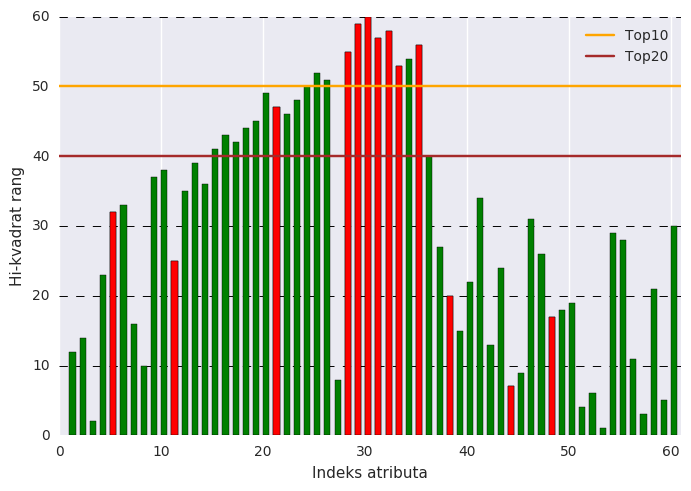
\includegraphics[height=12cm, width=16cm]{attributes}
    \caption[Grafički prikaz odabira atributa]{\textbf{Grafički prikaz odabira atributa rangiranih Hi-kvadrat testom.}  \textit{Iznad narančaste linije nalazi se najboljih 10 atributa, a iznad smeđe najboljih 20 atributa po Hi-kvadrat testu. Crvenom su označeni atributi izabrani korištenjem višeslojnog perceptrona.}}
    \label{fig:attributes}
\end{figure}
\begin{figure}[!ht]
    \centering
    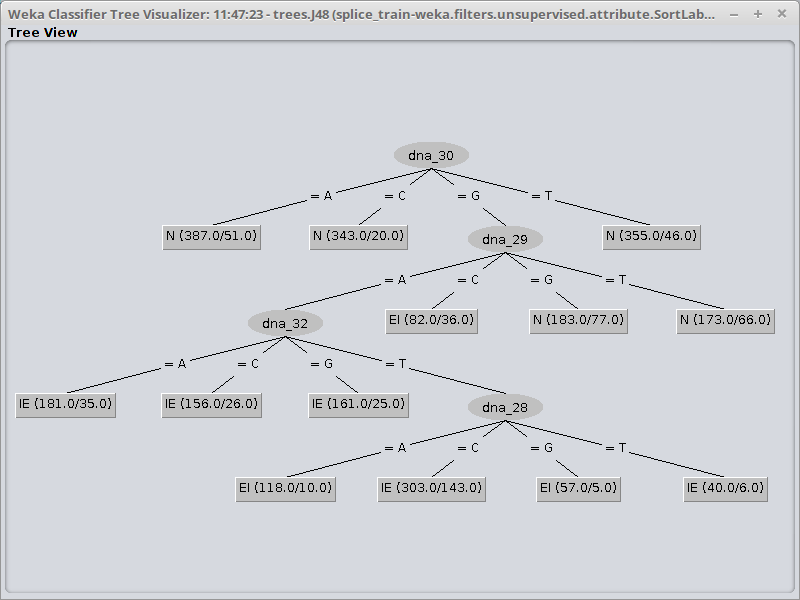
\includegraphics[height=15cm, width=16cm]{C45M100}
    \caption[Primjer modela stabla odlučivanja]{\textbf{Stablo odlučivanja - Weka model}  \textit{Stablo je stvoreno korištenjem skupa podataka sa svim atributima (model C4.5All) s minimalnim brojem objekata u podgrupi \textit{minNumObj} podešenim na 100. Ovakav model ima značajno nižu točnost (oko 80\%) u odnosu na modele u tablici \ref{tab:mjera}}}
    \label{fig:C45M100}
\end{figure}

Jedna od najvećih kvaliteta algoritma C4.5 je mogućnost iščitavanja značajki skupa podataka iz dobivenog modela (stabla). Slika \ref{fig:C45M100} prikazuje jedan mogući model. Odabran je velik stupanj podrezivanja zbog preglednosti. Zbog toga ovaj model obuhvaća samo četiri atributa. Stablo interpretiramo na slijedeći način. U korijenu stabla je \textit{dna{\_}30} atribut. Gledamo koji je nukleotid na toj poziciji u instanci. Ako se na toj poziciji ne nalazi nukleotid G, onda instanca ne predstavlja nukleotidni niz koji pripada akceptorskoj (klasa IE) odnosno donorskoj grupi (klasa EI). Ako se na toj poziciji nalazi nukleotid G, onda gledamo sadržaj atributa \textit{dna{\_}29}. Nukleotidi G i T na ovoj lokaciji znače da se ne radi niti o akceptorskoj niti o donorskoj sekvenci. Ako je na toj lokaciji nukleotid C, instancu svrstavamo u donorsku skupinu. Ako je vrijednost atributa A provjeravamo dalje vrijednost atributa \textit{dna{\_}32}. Ako je vrijednost ovog atributa T nastavljamo s provjerom atributa \textit{dna{\_}28} inače je instanca klase IE. Konačno atribut na lokaciji 28 je posljedni i on svrstava instancu u klase EI (ako je vrijednost atributa A ili G) i IE (ako je vrijednost atributa C ili T).

